\documentclass[12pt]{article}

\usepackage[english]{babel}
\usepackage[utf8x]{inputenc}
\usepackage{amsmath}
\usepackage{enumitem}
\usepackage{graphicx}
\usepackage{ulem}
\usepackage{caption}
\usepackage{placeins}
\usepackage[usenames,dvipsnames]{color}
\usepackage[colorinlistoftodos]{todonotes}
\usepackage{listings}
\usepackage{fixltx2e}
\usepackage{scrpage2}
\usepackage{lastpage}
\usepackage{glossaries}

\clearscrheadfoot
\pagestyle{scrheadings}
\usepackage[
top    = 2.75cm,
bottom = 2.00cm,
left   = 2.50cm,
right  = 2.00cm]{geometry}
\setcounter{secnumdepth}{4}

\begin{document}
\begin{titlepage}
\begin{center}
% Oberer Teil der Titelseite:

\includegraphics[width=0.9\textwidth]{images/vwlogo}\\[1cm]    


% Title
\rule{1.0\textwidth}{1mm}
{ \huge \bfseries \\[0.4cm]  \huge ERP-Evaluation \\[0.4cm] }
\LARGE TGM - HTBLuVA Wien XX \\ IT Department  \\[0.4cm]

\rule{1.0\textwidth}{1mm}




% Author and supervisor
\noindent 
\vspace{3cm}

\begin{center}
\large
Authors: \\ 
Bergler \textsc{Adrian} \&
Haidn \textsc{Martin} \&
Siegel \textsc{Hannah} \&
Soyka \textsc{Wolfram}
\end{center}

\vfill

% Bottom of the page
{\large \today}

\end{center}
\end{titlepage}

\tableofcontents


%HEADER AND FOOTER
\pagenumbering{arabic}
\ohead{\headmark}
\automark{section}
\ifoot{© Bergler, Haidn, Siegel, Soyka}
\ofoot{\pagemark ~of \pageref{LastPage}}

\newpage

\section{Auswahl des Unternehmens}

\section{Volkswagen AG}
http://www.economist.com/node/21558269
\subsection{Das Unternehmen}
\subsubsection{Historie}

\subsection{Finanzen}
%  3 u 4
\textbf{Umsatz}\\
Im Jahr 2013 lag der Umsatzerlös bei 65.587 Millionen Euro. Im Jahr zuvor jedoch betrug dieser 68.361 Millionen Euro. Ein Rückgang von 226 Millionen Euro ist dadurch entstanden. Gleichzeitig ist auch ein Gewinnrückgang von mehr als 3 Milliarden Euro festzuhalten. Gründe dafür lassen sich wie folgt finden:
\\
"Die in Vorjahren erworbenen 73,7\% der Anteile am Grundkapital der MAN SE, München, (9,1 Mrd.\euro) wurden von
der Volkswagen AG im Geschäftsjahr in die Truck \& Bus GmbH, eine 100-prozentige Tochtergesellschaft eingebracht.
Zusätzlich hat die Volkswagen AG 3,3 Mrd.\euro in die Kapitalrücklage der Truck \& Bus GmbH eingezahlt. Von der Truck \&
Bus GmbH wurden 2013 insgesamt 1,0 Mrd. \euro Verluste aufgrund des Beherrschungs- und Gewinnabführungsvertrags
mit der MAN SE übernommen. ",\cite[Seite 3]{jbilanz2013vw}
\\\\
"Die Volkswagen AG hat von der Volkswagen Bank GmbH, Braunschweig, eine Beteiligung erworben und diese anschließend im Wege der Sacheinlage (1,7 Mrd.\euro) in die VW Finance Luxemburg S.A., Luxemburg, eingebracht.\\
Darüber hinaus wurden Kapitalzuführungen bei der AUDI AG, Ingolstadt, (1,9 Mrd.\euro) und kleinere Kapitalmaß-
nahmen bei verbundenen Unternehmen durchgeführt. Bei der der Global Automotive C.V. Amsterdam, Niederlande
wurde eine Sachkapitalherabsetzung. (1,1 Mrd.\euro) durchgeführt. Die Volkswagen AG hat im HI-TV Fonds (TreasuryFonds) 1,0 Mrd.€ angelegt. ",\cite[Seite 4]{jbilanz2013vw}
\\ \\ 
\textbf{Aktie} \\
"On 7 April 1961, the Volkswagen Share was traded for the first time on a regulated open market, thus writing a chapter of economic history.",\cite{vsc50y} \\
\\
Marktkap. total (Stamm + Vorzug): EUR 114,71 Mrd.
\begin{figure}[here!]
\centering
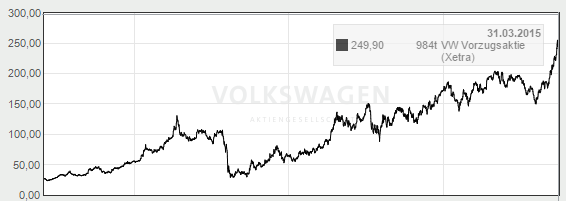
\includegraphics[width=0.7\textwidth]{images/finanzen2015}
\caption{Zehn Jahres Übersicht der VW-Vorzugsaktie \cite{aktienfotos}}
\label{fig:vwaktie1}
\end{figure}\FloatBarrier
\noindent
Wie in Abbildung \ref{fig:vwaktie1} zu sehen ist, ist die Volkswagen Vorzugsaktie in den letzten zehn Jahren stetig gestiegen. In 2008 wurde der Fall der Aktie durch die Finanzkrise bedingt.\\
Der Stand am Dienstag, dem 31. März 2015, der VW Vorzugsaktie (Xetra) war bei 249,90 \euro.
\begin{figure}[here!]
\centering
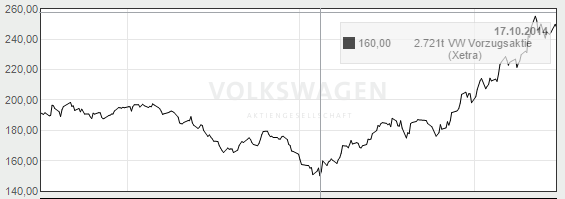
\includegraphics[width=0.7\textwidth]{images/finanzen20151}
\caption{Jahres Übersicht der VW-Aktie \cite{aktienfotos}}
\label{fig:vwaktie3}
\end{figure}\FloatBarrier
\noindent
Im letzten Jahr war das minimum im Oktober bei 160 \euro erreicht. Seit diesem Tag ist sie auch stetig bis auf kleine Ausnahmen gestiegen.
\begin{figure}[here!]
\centering
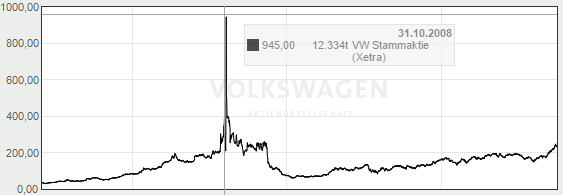
\includegraphics[width=0.7\textwidth]{images/finanzen2015S}
\caption{Zehn Jahres Übersicht der VW-Stammaktie \cite{aktienfotos}}
\label{fig:vwaktie2}
\end{figure}\FloatBarrier
\noindent
%TODO mama fragen
%(Reuters) - Volkswagen (VOWG.DE) briefly became the world's biggest company by market value on Tuesday, as short sellers caught betting on a price drop with borrowed stock scrambled to find shares after a buying spree by Porsche (PSHG_p.DE).Short sellers desperate to close their positions paid as much as 1,005 euros a share during the session following Sunday's news that there was less than 6 percent of VW voting stock still floating in the market.At that price Volkswagen's voting stock was worth 296 billion euros ($370 billion), or more than the $343 billion market capitalization of Exxon Mobil (XOM.N). VW shares later closed trading on Tuesday up 82 percent at 945 euros.
% % % \cite{2008wtf} % % %
\textbf{Aktinonärsstruktur}\\
Mit 31.12.2014 waren insgesammt 180.641.478 Vorzugsaktien und 295.089.818 Stammaktien ausstehend.\\
Im Juni 2014 hat die Volkswagen Aktiengesellschaft 10.471.204 neue Vorzugsaktien ausgegeben. Zusätzlich wurden im 1. Halbjahr 2014 22.103 Vorzugsaktien aus der Wandlung von Pflichtwandelanleihen geschaffen. Zum Stichtag 30. Juni 2014 setzte sich das gezeichnete Kapital der Volkswagen Aktiengesellschaft aus 295.089.818 Stammaktien und 180.641.478 Vorzugsaktien zusammen.
\cite{aktionaersstruktur} \\ \\
\textit{Stimmrechtsverteilung} \\
50,73\% Porsche Automobil Holding SE, Stuttgart\\
20,00\% Land Niedersachsen, Hannover\\
17,00\% Qatar Holding LLC\\
12,30\% Weitere
\\ \\
\textbf{Recovery}\\
"When Ferdinand Piëch arrived as Volkswagen's chief executive in 1993, things looked dire. The carmaker was overspending, overmanned and inefficient, and had lost its reputation for quality. How things have changed: last year the VW group's profits more than doubled, to a record €18.9 billion (\$23.8 billion). As other European volume carmakers seek to close factories and cut jobs, VW is seizing market share in Europe, booming in China and staging a comeback in America. It plans to spend €76 billion on new models and new factories by 2016. Its global workforce is more than half a million, and growing."\cite{ec2}
\\ \\
\textbf{Sales in America} \\
"The firm reported some of its best sales figures since the era of the original Beetle—and said it wanted to sell at least 800,000 vehicles per year in America by 2018.\\
Then, rather suddenly, things went south. Although Volkswagen of America is still well ahead of where it was before the Great Recession, it has suffered two consecutive years of declining sales. And in the first five months of 2014, as rivals such as GM posted some of their best numbers in a decade, the VW brand’s sales dropped by another 15\%. With sales in America barely above 400,000 in 2013, down 7\% from the previous year, doubts have been growing as to whether VW will be able to reach its target of 800,000 by 2018." \cite{ec1}

\begin{table}[h]
\begin{tabular}{|p{0.4\textwidth}|p{0.4\textwidth}|}
\hline
\textbf{Geschäftsjahr}  & \\  \hline
Geschäftsjahresende &   31. Dez \\  
Letztes Quartal (mrq) &   31.12.2014 \\  
Geschäftsjahresende &   31. Dez \\  \hline
\textbf{Rentabilität}  & \\  \hline
 Gewinnspanne (ttm)&   5,89\% \\  
 Operative Marge (ttm)&	5,89\%    \\ \hline
 \textbf{Managementeffektivität}  & \\  \hline
Kapitalrentabilität (ttm) & 2,21\%  \\  
Eigenkapitalrendite (ttm) &   12,28\%  \\  \hline
 \textbf{GuV}  & \\  \hline

 Umsatz (ttm)&   202,46Mrd. \\  
 Umsatz pro Aktie (ttm)&  408,12  \\  
 
Vierteljährliches Umsatzwachstum (yoy)&   6,60\% \\  
 Bruttoergebnis vom Umsatz (ttm)&34,39Mrd.    \\  
EBITDA (ttm)6 &  20,50Mrd.  \\  
 Auf Stammaktien entfallender Jahresüberschuss (ttm) &  10,98Mrd.  \\  \hline
  \textbf{Bilanz}  & \\  \hline


Cash (gesamt) (mrq): &  	28,30Mrd.  \\  

Gesamt-Cash pro Aktie (mrq): & 59,50   \\  
Schulden (gesamt) (mrq): &   108,65Mrd. \\  
 Schulden/Equity (gesamt) (mrq):&  	120,47  \\  \hline
   \textbf{Cash Flow-Aufstellung}  & \\  \hline

Cash Flow aus betrieblichen Tätigkeiten (ttm) &  10,78Mrd.  \\  
Levered Free Cash Flow (ttm) &  8,45Mrd.  \\  \hline

\end{tabular}
\end{table}
\cite{yahoofinanzenvw}













\subsection{Produktspektrum}
Das Produktspektrum der Volkswagen AG beinhaltet alle Kfz vom Stadtfahrzeug bis zum Großtransporter.

\subsection{Standorte und Unternehmensstruktur}
Volkswagen ist mit über 48 Niederlassungen in den folgenden Ländern vertreten:

\begin{table}[h]
	\begin{tabular}{|l|l|l|l|l|}
		\hline
		Argentinien          & Bosnien und Herzegovina & Brasilien & China    & Deutschland          \\ \hline
		Indien               & Mexiko                  & Polen     & Portugal & Russische Föderation \\ \hline
		Slowakische Republik & Spanien                 & Südafrika & USA      &                      \\ \hline
	\end{tabular}
\end{table}

Die Makre Volkswagen selbst Teilt sich in die Produktion von Kraftfahrzeugen für den Endverbraucher, sowie Nutzfahrzeuge für Privatkunden und Unternehmen.

\subsection{Logistik}
\subsection{Aufbau- und Ablauforganisation}
\subsection{Markt}
%Marktumfeld, -situation, -wert, Trends
Die Volkswagen Group, also alle Untermarken von VW gemeinsam produziert global am meisten KFZs (passenger cars?) 
In 2013 wurden etwa 9.3 Millionen Autos produziert. 
%In 2009, the global automotive industry was hit hard by the financial crisis of 2008-2009. Passenger car demand decreased in most regions, with the exception of emerging markets. Here, a growing middle class was becoming increasingly affluent and mobile. 
Der Level der 
Today, the volume of passenger cars produced is back to pre-crisis levels thanks to increased demand from both mature and emerging markets. VW, Toyota, Hyundai and GM were ranked as the largest manufacturers of passenger cars worldwide in 2013. While Germany’s VW and Japan’s Toyota are projected to generate healthy profits for years to come, General Motors is currently finding itself in midst of troubled times. In 2014, the U.S. automaker was forced to announce recalls of several million vehicles over a defective switch that has been linked to over 30 accidents and more than a dozen deaths. However, America’s largest car company has proven remarkably resilient before, when it fought its way back from bankruptcy and filed for an initial public offering (IPO) in 2010 following a company restructuring. In 2013, the Michigan-based company set a sales record in China, the largest passenger car market worldwide, and the carmaker is expected to perform well in China and North America over the next couple of years.


Manufacturer
Production in thousand units
9,259.51
8,565.18
6,909.19
6,733.19
4,263.24
4,090.68
3,317.05
2,452.57
2,445.89
2,347.91
2,163.04
2,006.37
1,685.39
1,631.5
1,175.44
VolkswagenToyotaHyundaiG.M.HondaNissanFordSuzukiPSARenaultFiatBMWSAICDaimler AGMazda


Source: 

© Statista 2015
http://www.statista.com/statistics/198524/15-leading-passenger-car-manufacturers-worldwide/



\subsection{Ziele und Zukunftsaspekte}

"Volkswagen has its eye on emerging markets with the new e-Golf, a version of its ever-popular hatchback line, as well as the smaller e-Up! “The empire strikes back,” proclaimed Heinz-Jakob Neusser, as the two models rolled onto the stage at a launch event during the media-preview days in Frankfurt. Europe’s largest carmaker now says it wants to have 40 hybrids, plug-ins and BEVs in the showrooms of its dozen brands by 2018. This represents a big shift: at the beginning of the decade the firm’s senior executives were still dismissing battery technology.",\cite{ec3}

"VOLKSWAGEN is nothing if not ambitious: its plan is to dethrone Toyota as the world’s biggest carmaker. It has already nosed past rival General Motors and has plenty of momentum in China, the world’s largest car market. But one key country is holding back the German giant: America.", \cite{ec1}
\section{Auswahl eines ERP Systemes}
\section*{Projekthandbuch}
\section*{Pflichtenheft}
\section*{Vorbereitung Kick Off Meeting}




\newpage
\listoftables
\listoffigures
\subsection{Easy Bibliography}
\begin{thebibliography}{56}

\bibitem{name}
%TODO
   \textbf{Who}, When\\
  \textit{url}
  \newline last used: dd.mm.yyyy, hh:mm
 
 \bibitem{ec1} 
  \textbf{Beetling back to success}, Jun 24th 2014, P.E, The Economist\\
  \textit{http://www.economist.com/blogs/schumpeter/2014/06/volkswagen-america}
  \newline last used: 07.03.2015, 13:00
  
   
 \bibitem{ec2} 
  \textbf{VW conquers the world - Germany’s biggest carmaker is leaving rivals in the dust}\\, Jul 7th 2012 , The Economist\\
  \textit{  http://www.economist.com/node/21558269}
  \newline last used: 07.03.2015, 13:07
  
    
   
 \bibitem{ec3} 
  \textbf{Europe goes electric - The Frankfurt motor show
}\\,Sep 12th 2013 , P.E., The Economist\\
  \textit{  http://www.economist.com/node/21558269}
  \newline last used: 07.03.2015, 13:09
  
   \bibitem{vsc50y} 
  \textbf{Volkswagen Share celebrates its 50th birthday}\\, Jun 4th 2011 , Volkswagen AG\\
  \textit{http://www.volkswagenag.com/content/vwcorp/info\_center/en/themes/2011/04/Volkswagen\_Share\_celebrates\_its\_50th\_birthday.html
}
  \newline last used: 07.03.2015, 13:16
  
   \bibitem{2008kurs} 
  \textbf{Volkswagen Share celebrates its 50th birthday}\\, Jun 4th 2011 , Volkswagen AG\\
  \textit{  http://www.boerse.de/boersenwissen/boersengeschichte/Kurskapriolen-der-VW-Aktie-2008-\%7C45}
  \newline last used: 07.03.2015, 13:24
  

   \bibitem{jbilanz2013vw} 
  \textbf{ABSCHLUSS VOLKSWAGEN AG }, 2013 \\
  \textit{ http://www.volkswagenag.com/content/vwcorp/info\_center/de/publications/2014/03/Financial\_Statements\_VWAG\_2013.bin.html/binarystorageitem/file/Abschluss+Volkswagen+AG+2013\_deutsch.pdf  
}
  \newline last used: 08.03.2015, 14:03
    
    
       \bibitem{aktionaersstruktur} 
  \textbf{Aktionärsstruktur Volkswagen AG}, Stand 31.12.2014 \\
  \textit{http://www.volkswagenag.com/content/vwcorp/content/de/investor\_relations/share/Shareholder\_Structure.html}
  \newline last used: 01.04.2015, 15:04
  
       \bibitem{2008wtf} 
 \textbf{Short sellers make VW the world's priciest firm}, reuters.com. SARAH Marsh \\
  \textit{  http://www.reuters.com/article/2008/10/28/us-volkswagen-idUSTRE49R3I920081028}
  \newline last used: 01.04.2015, 15:39  
  
         \bibitem{aktienfotos} 
 \textbf{Vorzugs- und Stammaktien}, volkswagenag.com \\
  \textit{   http://www.volkswagenag.com/content/vwcorp/content/de/investor\_relations/share.html}
  \newline last used: 01.04.2015, 15:57  
  
      \bibitem{yahoofinanzenvw} 
 \textbf{Volkswagen AG},Yahoo Finanzen \\
  \textit{  https://de.finance.yahoo.com/q/ks?s=VOW3.DE}
  \newline last used: 01.04.2015, 16:33  
    
\end{thebibliography}
\end{document}
%img : httpmarkets.ft.comresearchMarketsTearsheetsSummarys=VOWBER vwdax.PNG